%% abtex2-modelo-trabalho-academico.tex, v-1.9.2 laurocesar
%% Copyright 2012-2017 by abnTeX2 group at http://abntex2.googlecode.com/ 
%%
%% This work may be distributed and/or modified under the
%% conditions of the LaTeX Project Public License, either version 1.3
%% of this license or (at your option) any later version.
%% The latest version of this license is in
%%   http://www.latex-project.org/lppl.txt
%% and version 1.3 or later is part of all distributions of LaTeX
%% version 2005/12/01 or later.
%%
%% This work has the LPPL maintenance status `maintained'.
%% 
%% The Current Maintainer of this work is Emílio Eiji Kavamura,
%% eek.edu@outlook.com; emilio.kavamura@ufpr.br
%% Further information about abnTeX2 are available on 
%%
%% http://abntex2.googlecode.com/
%%
%% https://code.google.com/p/abntex2/issues/ 
%%
%% Further information about UFPR abnTeX2 are available on 
%%
%% https://github.com/eekBR/ufpr-abntex/
%%
%% This work consists of the files 
% 
%          main.tex   programa principal
%      00-dados.tex   entrada de dados 
%    00-pacotes.tex   pacotes carregados no modelo
% 00-pretextual.tex   processamento dos elementos pre-textuais
%          UFPR.sty   ajusta do modelo canonico às normas  UFPR
%
%    referencias.bib
%                     e outras arquivos de imagens
%
%
%------------------------------------------------------------------------
% ------------------------------------------------------------------------
% abnTeX2: Modelo de Trabalho Academico (tese de doutorado, dissertacao de
% mestrado e trabalhos monograficos em geral) em conformidade com 
% ABNT NBR 6023:2018: Informação e documentação - Referências - Elaboração
% ------------------------------------------------------------------------
% ------------------------------------------------------------------------
%
% DATA DE ATUALIZAÇÃO: 2020-06-10

\documentclass[
        % -- opções da classe memoir --
        12pt,                           % tamanho da fonte
        openright,                      % capítulos começam em pág ímpar (insere página vazia caso preciso)
        %twoside,                        % para impressão em verso e anverso. Oposto a oneside
        oneside,
        a4paper,                        % tamanho do papel. 
        % -- opções da classe abntex2 --
        chapter=TITLE,         % títulos de capítulos convertidos em letras maiúsculas
        section=TITLE,         % títulos de seções convertidos em letras maiúsculas
        subsection=Title,      % títulos de subseções convertidos em letras maiúsculas
        %subsubsection=TITLE,  % títulos de subsubseções convertidos em letras maiúsculas
        % -- opções do pacote babel --
        english,                        % idioma adicional para hifenização
        %french,                         % idioma adicional para hifenização
        spanish,                        % idioma adicional para hifenização
        portugues,                      % o último idioma é o principal do documento
        %%%%%%%%%%%%
        %eek: colocação da opção para o sumario ter formatação tradicional
        sumario=tradicional             % título no formato tradicional
        ]{abntex2}


\usepackage{UFPR}
% Pacotes básicos 
% ----------------------------------------------------------
\usepackage{lmodern}			% Usa a fonte Latin Modern			
\usepackage[T1]{fontenc}		% Selecao de codigos de fonte.
\usepackage[utf8]{inputenc}		% Codificacao do documento (conversão automática dos acentos)
\usepackage{lastpage}			% Usado pela Ficha catalográfica
\usepackage{indentfirst}		% Indenta o primeiro parágrafo de cada seção.
\usepackage{color}		    	% Controle das cores
\usepackage{graphicx}			% Inclusão de gráficos
\usepackage{microtype} 			% para melhorias de justificação
\usepackage{ifthen}		    	% para montar condicionais
\usepackage[brazil]{babel}		% para utilizar termos em portugues
\usepackage[final]{pdfpages}    % para incluir páginas de arquivos pdf
\usepackage{lipsum}				% para geração de dummy text
\usepackage{csquotes}

%\usepackage[style=long]{glossaries}
%\usepackage{abntex2glossaries}

\usepackage{algorithm} 
\usepackage{algpseudocode} 
\usepackage{cancel} 		% permite representar o cancelamento de termos em texto ou equacoes	
\usepackage{xcolor} 		% cores extendidas	
\usepackage{smartdiagram}   	% gera diagramas a partir de listas
%\usepackage{float} 		% Para a figura ficar na posição correta	    
\usepackage{textcomp} 		% supporte para fontes da Text Companion 
\usepackage{longtable}		% uso de longtable
\usepackage{amsmath}		% simbolos matematicos
\usepackage{lscape}		% páginas em paisagem
\usepackage{multicol}		% mescla de colunas em tabelas
\usepackage{multirow}		% mescla de linhas em tabelas
\usepackage{newfloat} 		% criação do indice de quadros
%\usepackage{caption} 		% configura legenda 
	%[format=plain]
	%\renewcommand\caption[1]{%
    	%\captionsetup{font=small}	% tamanho da fonte 10pt
    	%,format=hang
 	% \caption{#1}}
	%\captionsetup{width=0.8\textwidth}
\captiondelim{-- }
\captiontitlefont{\small}
\captionnamefont{\small}

\definecolor{dkgreen}{rgb}{0,0.6,0}
\definecolor{gray}{rgb}{0.5,0.5,0.5}
\definecolor{mauve}{rgb}{0.58,0,0.82}

% Pacotes de citações BibLaTeX
% ----------------------------------------------------------
\usepackage[style=abnt,
	backref=true,
	backend=biber,
	citecounter=true,
	backrefstyle=three, 
	url=true,
	maxbibnames=99,
    mincitenames=1,
    maxcitenames=2,
    backref=true,
    hyperref=true,
    firstinits=true,
    uniquename=false,
    uniquelist=false]{biblatex}
    
% Espaçamento entre os itens nas referências (espço de uma linha simples)
% ----------------------------------------------------------
\setlength\bibitemsep{\baselineskip}

% Texto padrão para as referências
% ----------------------------------------------------------
\DefineBibliographyStrings{brazil}{%
	 backrefpage  = {Citado \arabic{citecounter} vez na página},		% originally "cited on page"
	 backrefpages = {Citado \arabic{citecounter} vezes nas páginas},	% originally "cited on pages"
	 urlfrom      = {Dispon\'ivel em},
}

% Ajusta indentação de Referencias no ToC
% ----------------------------------------------------------
\defbibheading{bay}[\bibname]{%
  \chapter*{#1}%
  \markboth{#1}{#1}%
  \addcontentsline{toc}{chapter}
  {\protect\numberline{}\bibname}
}

% Formatando o avançao dos títulos no sumário 
% ----------------------------------------------------------
\makeatletter
	\pretocmd{\chapter}{\addtocontents{toc}{\protect\addvspace{-12\p@}}}{}{}
	\pretocmd{\section}{\addtocontents{toc}{\protect\addvspace{-3\p@}}}{}{}
\makeatother

% Para retirar os símbolos <> da URL  
% ----------------------------------------------------------
\DeclareFieldFormat{illustrated}{\addspace #1\isdot}%
%\DeclareFieldFormat{url}{\bibstring{urlform}\addcolon\addspace<\url{#1}>}%
%\DeclareFieldFormat{url}{\bibstring{urlfrom}\addcolon\addspace<\url{#1}>}%
\DeclareFieldFormat{url}{\bibstring{urlfrom}\addcolon \space\addspace{#1}} 
% remove <> em urls de acordo com abnt-6023:2018	

% Ajustar o espaço para a formatação da data
% ----------------------------------------------------------
\DeclareFieldFormat{urldate}{\bibstring{urlseen}\addcolon\addspace #1}%
\DeclareFieldFormat*{note}{\addspace #1}%

% Para ajustar o tamanho da fonte do número da primeira página do capítulo
% comando utilizado na parte textual 
% ----------------------------------------------------------
\makepagestyle{chapfirst}% Just for the first page of a chapter
\makeoddhead{chapfirst}{}{}{\footnotesize{\thepage}}

%%criar um novo estilo de cabeçalhos e rodapés
\makepagestyle{simplestextual}
  %%cabeçalhos
  \makeevenhead{simplestextual} %%pagina par
     {}{}{\footnotesize \thepage}
     
  \makeoddhead{simplestextual} %%pagina ímpar ou com oneside
     {}{}{\footnotesize \thepage}
  %\makeheadrule{simplestextual}{\textwidth}{\normalrulethickness} %linha
  %% rodapé
  \makeevenfoot{simplestextual}
     {}{}{} %%pagina par
      
  \makeoddfoot{simplestextual} %%pagina ímpar ou com oneside
     {}{}{}
     
% Define a formatação dos capítulos póstextuais numerados
% ----------------------------------------------------------
\newcommand{\poschap}[1]{
	\stepcounter{chapter}
	\markboth{#1}{#1}%
	\pdfbookmark[2]{#1}{#1}
	\addtocontents{toc}{\vspace{-0pt}}
	\addcontentsline{toc}{chapter}{\hspace{14.5mm}\textbf{\appendixname~
	\thechapter~- #1}}
	\chapter*{\appendixname\space\space\thechapter~- \uppercase{#1}}%
	{}
}
\newcommand{\refap}[1]{\hyperref[#1]{Apêndice~\ref{#1}}} 	% Referência apÊndices
% uso do tikz e pgfplots
% ----------------------------------------------------------
%\usetikzlibrary{external}
\usetikzlibrary{arrows,calc,patterns,angles,quotes}
\usepackage{pgfplots}
\pgfplotsset{compat=1.15}

% Define o comando para citação de fontes em elementos gráficos (figuras, imagens,...).
% ----------------------------------------------------------
%  AUTOR(ano)
%
% parâmetro é a bibkey da fonte
  
\newcommand{\citefig}[2]{~\Citeauthor*{#1}\citeyear{#1}}

% Define os operadores matemáticos em portugues
% ----------------------------------------------------------
%

\DeclareMathOperator{\tr}{tr}
\DeclareMathOperator{\sen}{sen}
\DeclareMathOperator{\senh}{senh}
%\DeclareMathOperator{\tag}{tag}
\DeclareMathOperator{\tg}{tg}
\DeclareMathOperator{\tagh}{tagh}
\DeclareMathOperator{\tgh}{tgh}
\DeclareMathOperator{\cossec}{cossec}
%\DeclareMathOperator{\sen}{sen}

% Para fazer a listagem de codigos LaTeX na documentação
% ----------------------------------------------------------
\usepackage{listings}

%Comando para fazer 
%    a citação de documentos não publicados e informais e 
%    colocar as referências nas notas de rodapé
% ----------------------------------------------------------

\newcommand{\citenp}[1]{
\cite{#1}\footnote{\fullcite{#1}}}

\newcommand{\textcitenp}[1]{
	\textcite{#1}\footnote{\fullcite{#1}}}
%%%%%%%%%%%%%%%%%%%%%%%%%%%%%%%%%%%%%%%%%%%%%%%%%%%%%%%
% Arquivo para entrada de dados para a parte pré textual
%%%%%%%%%%%%%%%%%%%%%%%%%%%%%%%%%%%%%%%%%%%%%%%%%%%%%%%
% 
% Basta digitar as informações indicidas, no formato 
% apresentado.
%
%%%%%%%
% Os dados solicitados são, na ordem:
%
% tipo do trabalho
% componentes do trabalho 
% título do trabalho
% nome do autor
% local 
% data (ano com 4 dígitos)
% orientador(a)
% coorientador(a)(as)(es)
% arquivo com dados bibliográficos
% instituição
% setor
% programa de pós gradução
% curso
% preambulo
% data defesa
% CDU
% errata
% assinaturas - termo de aprovação
% resumos & palavras chave
% agradecimentos
% dedicatoria
% epígrafe


% Informações de dados para CAPA e FOLHA DE ROSTO
%----------------------------------------------------------------------------- 
\tipotrabalho{Dissertação}
%    {Relatório Técnico}
%    {Dissertação}
%    {Tese}
%    {Monografia}
% {Trabalho Acadêmico}

% Marcar Sim para as partes que irão compor o documento pdf
%----------------------------------------------------------------------------- 
 \providecommand{\terCapa}{Sim}
 \providecommand{\terFolhaRosto}{Sim}
 \providecommand{\terTermoAprovacao}{Sim}
 \providecommand{\terDedicatoria}{Sim}
 \providecommand{\terFichaCatalografica}{Nao}
 \providecommand{\terEpigrafe}{Nao}
 \providecommand{\terAgradecimentos}{Sim}
 \providecommand{\terErrata}{Nao}
 \providecommand{\terListaFiguras}{Nao}
 \providecommand{\terListaQuadros}{Nao}
 \providecommand{\terListaTabelas}{Nao}
 \providecommand{\terSiglasAbrev}{Nao}
 \providecommand{\terResumos}{Sim}
 \providecommand{\terSumario}{Sim}
 \providecommand{\terAnexo}{Nao}
 \providecommand{\terApendice}{Nao}
 \providecommand{\terIndiceR}{Nao}
%----------------------------------------------------------------------------- 

\titulo{Titulo}
\autor{Maria Teresa Kravetz Andrioli}
\local{Curitiba}
\data{2022} %Apenas ano 4 dígitos

% Orientador ou Orientadora
\orientador{Prof. Dr. Luiz Carlos P. Albini}
%Prof Emílio Eiji Kavamura, MSc}
\orientadora{}
% Pode haver apenas uma orientadora ou um orientador
% Se houver os dois prevalece o feminino.

% Em termos de coorientação, podem haver até quatro neste modelo
% Sendo 2 mulhere e 2 homens.
% Coorientador ou Coorientadora
\coorientador{}%Prof Morgan Freeman, DSc}
\coorientadora{}

% Segundo Coorientador ou Segunda Coorientadora
\scoorientador{}
%Prof Jack Nicholson, DEng}
\scoorientadora{}
%Prof\textordfeminine~Ingrid Bergman, DEng}
% ----------------------------------------------------------
\addbibresource{referencias.bib}

% ----------------------------------------------------------
\instituicao{%
Universidade Federal do Paraná}

\def \ImprimirSetor{Setor de Ciências Exatas}%
%Setor de Tecnologia}

\def \ImprimirProgramaPos{}%Programa de Pós Graduação em Engenharia de Construção Civil}

\def \ImprimirCurso{Curso de Ciência da Computação}%
%Curso de Engenharia Civil}

\preambulo{
  Trabalho apresentado como requisito parcial para a obtenção do grau de Bacharel em Ciência da Computação no curso de Ciência da Computação, Setor de Ciências Exatas da Universidade Federal do Paraná}
%do grau de Bacharel em Expressão Gráfica no curso de Expressão Gráfica, Setor de Exatas da Universidade Federal do Paraná}

%----------------------------------------------------------------------------- 

\newcommand{\imprimirCurso}{}
%Programa de P\'os Gradua\c{c}\~ao em Engenharia da Constru\c{c}\~ao Civil}

\newcommand{\imprimirDataDefesa}{Maio de 2022}

\newcommand{\imprimircdu}{
02:141:005.7}

% ----------------------------------------------------------
\newcommand{\imprimirerrata}{
Elemento opcional da \cites[4.2.1.2]{NBR14724:2011}. Exemplo:

\vspace{\onelineskip}

FERRIGNO, C. R. A. \textbf{Tratamento de neoplasias ósseas apendiculares com
reimplantação de enxerto ósseo autólogo autoclavado associado ao plasma
rico em plaquetas}: estudo crítico na cirurgia de preservação de membro em
cães. 2011. 128 f. Tese (Livre-Docência) - Faculdade de Medicina Veterinária e
Zootecnia, Universidade de São Paulo, São Paulo, 2011.

\begin{table}[htb]
\center
\footnotesize
\begin{tabular}{|p{1.4cm}|p{1cm}|p{3cm}|p{3cm}|}
  \hline
   \textbf{Folha} & \textbf{Linha}  & \textbf{Onde se lê}  & \textbf{Leia-se}  \\
    \hline
    1 & 10 & auto-conclavo & autoconclavo\\
   \hline
\end{tabular}
\end{table}}

% Comandos de dados - Data da apresentação
\providecommand{\imprimirdataapresentacaoRotulo}{}
\providecommand{\imprimirdataapresentacao}{}
\newcommand{\dataapresentacao}[2][\dataapresentacaoname]{\renewcommand{\dataapresentacao}{#2}}

% Comandos de dados - Nome do Curso
\providecommand{\imprimirnomedocursoRotulo}{}
\providecommand{\imprimirnomedocurso}{}
\newcommand{\nomedocurso}[2][\nomedocursoname]
  {\renewcommand{\imprimirnomedocursoRotulo}{#1}
\renewcommand{\imprimirnomedocurso}{#2}}


% ----------------------------------------------------------
\newcommand{\AssinaAprovacao}{

\assinatura{%\textbf
   {Professora} \\ UFPR}
   \assinatura{%\textbf
   {Professora}}
   \assinatura{%\textbf
   {Professora}}
   %\assinatura{%\textbf{Professor} \\ Convidado 4}
      
   \begin{center}
    \vspace*{0.5cm}
    %{\large\imprimirlocal}
    %\par
    %{\large\imprimirdata}
    \imprimirlocal, \imprimirDataDefesa.
    \vspace*{1cm}
  \end{center}
  }
  
% ----------------------------------------------------------
%\newcommand{\Errata}{%\color{blue}
%Elemento opcional da \textcite[4.2.1.2]{NBR14724:2011}. Exemplo:
%}

% ----------------------------------------------------------
\newcommand{\EpigrafeTexto}{%\color{blue}
\textit{``Não vos amoldeis às estruturas deste mundo, \\
		mas transformai-vos pela renovação da mente, \\
		a fim de distinguir qual é a vontade de Deus: \\
		o que é bom, o que Lhe é agradável, o que é perfeito.\\
		(Bíblia Sagrada, Romanos 12, 2)}
}

% ----------------------------------------------------------
\newcommand{\ResumoTexto}{%\color{blue}
O resumo deve ressaltar o  objetivo, o método, os resultados e as conclusões do documento. A ordem e a extensão destes itens dependem do tipo de resumo (informativo ou indicativo) e do tratamento que cada item recebe no documento original. O resumo deve ser precedido da referência do documento, com exceção do resumo inserido no próprio documento. (\ldots) As palavras-chave devem figurar logo abaixo do  resumo, antecedidas da expressão Palavras-chave:, separadas entre si por ponto e finalizadas também por ponto.Ter no máximo 500 palavras!!! As palavras chave são separadas por ponto e vírgula.
} 

\newcommand{\PalavraschaveTexto}{%\color{blue}
latex; abntex; editoração de texto.}

% ----------------------------------------------------------
\newcommand{\AbstractTexto}{%\color{blue}
This is the english abstract.
}
% ---
\newcommand{\KeywordsTexto}{%\color{blue}
latex. abntex. text editoration.
}

% ----------------------------------------------------------
\newcommand{\Resume}
{%\color{blue}
%Il s'agit d'un résumé en français.
} 
% ---
\newcommand{\Motscles}
{%\color{blue}
 %latex. abntex. publication de textes.
}

% ----------------------------------------------------------
\newcommand{\Resumen}
{%\color{blue}
%Este es el resumen en español.
}
% ---
\newcommand{\Palabrasclave}
{%\color{blue}
%latex. abntex. publicación de textos.
}

% ----------------------------------------------------------
\newcommand{\AgradecimentosTexto}{%\color{blue}
Os agradecimentos principais são direcionados à Gerald Weber, Miguel Frasson, Leslie H. Watter, Bruno Parente Lima, Flávio de  Vasconcellos Corrêa, Otavio Real Salvador, Renato Machnievscz\footnote{Os nomes dos integrantes do primeiro
projeto abn\TeX\ foram extraídos de \url{http://codigolivre.org.br/projects/abntex/}} e todos aqueles que contribuíram para que a produção de trabalhos acadêmicos conforme as normas ABNT com \LaTeX\ fosse possível.

Agradecimentos especiais são direcionados ao Centro de Pesquisa em Arquitetura da Informação\footnote{\url{http://www.cpai.unb.br/}} da Universidade de Brasília (CPAI), ao grupo de usuários
\emph{latex-br}\footnote{\url{http://groups.google.com/group/latex-br}} e aos novos voluntários do grupo \emph{\abnTeX}\footnote{\url{http://groups.google.com/group/abntex2} e
\url{http://abntex2.googlecode.com/}}~que contribuíram e que ainda
contribuirão para a evolução do \abnTeX.

Os agradecimentos principais são direcionados à Gerald Weber, Miguel Frasson, Leslie H. Watter, Bruno Parente Lima, Flávio de Vasconcellos Corrêa, Otavio Real Salvador, Renato Machnievscz\footnote{Os nomes dos integrantes do primeiro
projeto abn\TeX\ foram extraídos de \url{http://codigolivre.org.br/projects/abntex/}} e todos aqueles que contribuíram para que a produção de trabalhos acadêmicos conforme as normas ABNT com \LaTeX\ fosse possível.
}

% ----------------------------------------------------------
\newcommand{\DedicatoriaTexto}{%\color{blue}
\textit{ Este trabalho é dedicado às crianças adultas que,\\
   quando pequenas, sonharam em se tornar cientistas.}
	}



% compila o indice
% ----------------------------------------------------------

\makeindex
% ----------------------------------------------------------
% Início do documento
% ----------------------------------------------------------
\begin{document}
% ----------------------------------------------------------
% Adequando o uppercase titulo dos elementos nas suas respectivas legendas
% Definicoes que n\~ao funcionaram quando colocados no arquivo de estilos ou de pacotes

\renewcommand{\bibname}{{REFER\^ENCIAS}}
\renewcommand{\tablename}{TABELA }
\renewcommand{\figurename}{FIGURA }
\renewcommand{\figureautorefname}{FIGURA}
\renewcommand{\tableautorefname}{TABELA}
\newcommand{\equationname}{EQUA\c{C}\~AO~}
\renewcommand{\equationautorefname}{EQUA\c{C}\~AO~}

% Para ajustar o tamanho da fonte do número da primeira página do capítulo
\aliaspagestyle{chapter}{chapfirst}% customizing chapter pagestyle

% ELEMENTOS PRÉ-TEXTUAIS
\makeoddhead{chapfirst}{}{}{}
% ----------------------------------------------------------
% Capa
% ----------------------------------------------------------
 \ifthenelse{\equal{\terCapa}{Sim}}{
\imprimircapa}{}

% Folha de rosto
% ----------------------------------------------------------
\imprimirfolhaderosto*

% Inserir a ficha bibliografica
% ----------------------------------------------------------
 \ifthenelse{\equal{\terFichaCatalografica}{Sim}}
 {\insereFichaCatalografica{}\cleardoublepage}
 {}

% Inserir errata
% ----------------------------------------------------------
 \ifthenelse{\equal{\terErrata}{Sim}}
 {\begin{errata}%\color{blue}
   \imprimirerrata
  \end{errata}}
 {}

% Inserir folha de aprovação
% ----------------------------------------------------------
\ifthenelse{\equal{\terTermoAprovacao}{Sim}}{
\insereAprovacao}{}

% Dedicatória
% ----------------------------------------------------------
\ifthenelse{\equal{\terDedicatoria}{Sim}}{
\begin{dedicatoria}
   \vspace*{\fill}
   \centering
   \noindent
   \DedicatoriaTexto
   \vspace*{\fill}
\end{dedicatoria}
}{}

% Agradecimentos
% ----------------------------------------------------------

 \ifthenelse{\equal{\terAgradecimentos}{Sim}}
 {\begin{agradecimentos}
    \AgradecimentosTexto
  \end{agradecimentos}
  }{}
% Epígrafe
% ----------------------------------------------------------

\ifthenelse{\equal{\terEpigrafe}{Sim}}{
\begin{epigrafe}
    \vspace*{\fill}
	\begin{flushright}
        \EpigrafeTexto
	\end{flushright}
\end{epigrafe}
}{}

% RESUMOS
% ----------------------------------------------------------
% resumo em português
%\setlength{\absparsep}{18pt} % ajusta o espaçamento dos parágrafos do resumo
 \ifthenelse{\equal{\terResumos}{Sim}}{
\begin{resumo}
    \ResumoTexto
    
    %\vspace{\onelineskip}
    \noindent 
    \textbf{Palavras-chaves}: \PalavraschaveTexto
\end{resumo}

%% resumo em inglês
\begin{resumo}[ABSTRACT]
 \begin{otherlanguage*}{english}
   \AbstractTexto
   
   %\vspace{\onelineskip}
   \noindent 
   \textbf{Key-words}: \KeywordsTexto
 \end{otherlanguage*}
\end{resumo}


% resumo em francês 
\ifthenelse{\equal{\Resume}{}}
{}
{
 \begin{resumo}[RESUME]%Résumé
  \begin{otherlanguage*}{french}
     \Resume
     
     %\vspace{\onelineskip}
     \noindent      
     \textbf{Mots clés}: \Motscles
  \end{otherlanguage*}
 \end{resumo}
} 

% resumo em espanhol
\ifthenelse{\equal{\Resume}{}}{}
{ \begin{resumo}[RESUMEN]
  \begin{otherlanguage*}{spanish}
    \Resumen 
   
   %\vspace{\onelineskip}
   \noindent    
    \textbf{Palabras clave}: \Palabrasclave
  \end{otherlanguage*}
 \end{resumo}
}
}{}

% inserir lista de ilustrações
% ----------------------------------------------------------
\ifthenelse{\equal{\terListaFiguras}{Sim}}{
%\pdfbookmark[0]{\listfigurename}{lof}
\listoffigures*
\cleardoublepage
}{}

% inserir lista de quadros
% ----------------------------------------------------------
\ifthenelse{\equal{\terListaQuadros}{Sim}}{
%\pdfbookmark[0]{\listtablename}{lot}
\listofquadros*
\cleardoublepage
}{}

% inserir lista de tabelas
% ----------------------------------------------------------
\ifthenelse{\equal{\terListaTabelas}{Sim}}{
%\pdfbookmark[0]{\listtablename}{lot}
\listoftables*
\cleardoublepage
}{}


% inserir lista de abreviaturas e siglas 
% inserir lista de símbolos
% ----------------------------------------------------------

 \ifthenelse{\equal{\terSiglasAbrev}{Sim}}{
    \imprimirlistadesiglas
    \cleardoublepage
    \imprimirlistadesimbolos
    \cleardoublepage
 }{}

% inserir o sumario
\makeoddhead{chapfirst}{}{}{}
% ----------------------------------------------------------
\ifthenelse{\equal{\terSumario}{Sim}}{
%\pdfbookmark[0]{\contentsname}{toc}
\tableofcontents*
%\cleardoublepage
}{}
 

 
 


% ----------------------------------------------------------
% ELEMENTOS TEXTUAIS
% ----------------------------------------------------------
\textual % \pagestyle{textualUFPR}

\pagestyle{simplestextual}
% sugerido por Youssef Cherem 20170316
% https://mail.google.com/mail/u/0/?tab=wm#inbox/15ad3fe6f4e5ff1f

% Introdução (exemplo de capítulo sem numeração, mas presente no Sumário)
% ----------------------------------------------------------
\chapter{INTRODUÇÃO} \label{cha:introd}

Esta é uma série para apresentar o uso do template e não uma documentação da customização. Este documento pressume que você conheça algumas características de uso do LaTeX, caso não tenha nenhuma informação/formação, basta acessar o documento de documentação em pdf deste repositório. Nele você encontrará um curso básico de LaTeX para utilizar a customização sem muitas dificuldades.

Claro, a curva de aprendizado inicial é difícil de ser percorrida. Depois de se acostumar, fica mais simples e satisfatório.
\section{UTILIZAÇÃO DESTE TEMPLATE} \label{sec:util}

Veja que é necessário colocar os títulos do capítulo e da seção em caixa alta. É recomendado ter um texto entre as seções do documento.

Você pode digitar o texto e utilizar os recursos do LaTeX para colocar os elementos gráficos, tabelas, quadros, expressões matemáticas, siglas, símbolos, citações e referências. Foram configurados alguns comandos para facilitar o seu trabalho.
\subsection[Imagens]{Imagens e figuras}\label{ssec:imafig}

Para inserir uma figura com o comando \verb+\includegraphics+ para ficar de acordo com a normalização ABNT-UFPR:
\subsubsection{imagem}\label{sssec:imagem}

\verb+\imagem{Título da imagem}{largura}+ 

\verb+   {figura com sua localização }{Fonteda figura}+

\verb+   {label}{alguma nota}{alguma legenda}+

\begin{lstlisting}
\figura
{FIGURA DE TIPOS PARA IMPRESSAO}  % Titulo
{.75}                             % % da largura da linha
{fig/tipog.png}                   % caminho da figura
{\citefig{tipo2012}.}             % Fonte
{tipoex}                          % label = fig:tipoex
{Esta eh uma nota musical, 
 Esta eh uma nota musical e 
 Esta eh uma outra nota}          % Texto da Nota
{Nao quero colocar legenda.}      % Texto da Legenda
\end{lstlisting}

Para fazer referencia a esta figura, basta digitar \verb+\autoref{fig:tipoex}+.

Para inserir um elemento gráfico gerado/compativel com o LaTeX, você tem o comando imagem com 7 parâmetros:

\begin{lstlisting}
% simplificacao para colocar figuras
% ----------------------------------------------------------
%   Parametros
%    1 caption
%    2 percent textwidth
%    3 arquivo da figura
%    4 fonte
%    5 fig:label
%    6 nota
%    7 legenda

\figura
{FIGURA DE TIPOS PARA IMPRESSAO}  % Titulo
{.750}                            % %da largura da linha
{fig/tipog.png}                   % caminho da figura
{\citefig{tipo2012}.}             % Fonte
{tipoex}                          % label = fig:tipoex
{Esta eh uma nota musical. 
 Esta eh uma nota musical.
 Esta eh uma nota musical. 
 Esta eh uma nota e esta 
	eh uma outra nota}            % Texto da Nota
{Nao quero colocar legenda.}      % Texto da Legenda
\end{lstlisting}

Para fazer referência a esta figura, basta digitar \verb+\autoref{fig:tipoex}+

\begin{lstlisting}
% simplificacao para colocar imagens
% ----------------------------------------------------------
%   Parametros
%    1 caption
%    2 imagem tikz ou pgfplots ou outro elemento qualquer
%    3 fonte
%    4 fig:label
%    5 nota
%    6 legenda
\end{lstlisting}

\verb+\imagem{Titulo}{arg2}{fonte}{label}{nota(s)}{legenda(s)}+

\begin{lstlisting}
\imagem{Titulo}
	{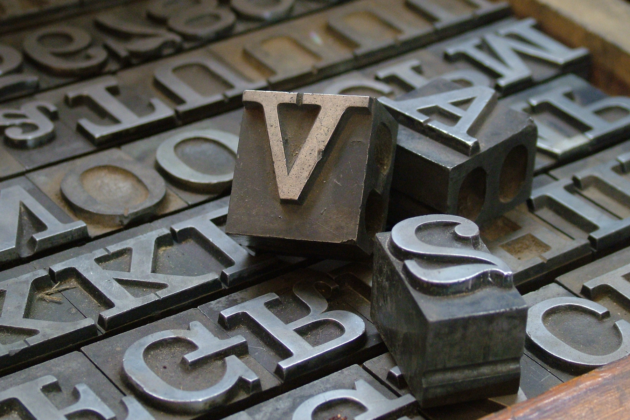
\includegraphics[width = 80mm]{fig/tipog}}
	{fonte}
	{label}
	{nota(s)}
	{legenda(s)}
\end{lstlisting}


\imagem{Titulo}{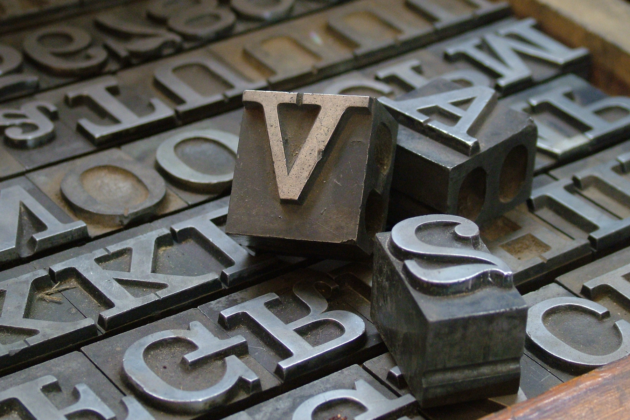
\includegraphics[width = 80mm]{fig/tipog}}{fonte}{label}{nota(s)}{legenda(s)}

Para fazer referência a esta figura é da mesma forma,\verb+\autoref{fig:label}+, \autoref{fig:label}

\subsection[Quadros e tabelas]{Quadros e tabelas}

Lembrando que quadros tem informações e são fechados lateralmente e verticalmente, tem a posição do título, fonte, nota e legenda diferentes da tabela.
\subsection[Quadros]{Inserir quadros}\label{ssec:quadros}

Para inserir um quadro são necessários 6 parâmetros:

\begin{lstlisting}
% ----------------------------------------------------------
%   Parametros
%    1 caption
%    2 elementos tabulados
%    3 fonte
%    4 qua:label
%    5 nota
%    6 legenda
\end{lstlisting}

Os elemento tabulados foram inseridos no ambiente tabular, com as laterais e parte superior e inferior fechados.

Este ambiente não quebra sua estrutura em páginas.

\begin{lstlisting}
\qquadro{Prefixos convencionados para referencias}
{\footnotesize
 \begin{tabular}{|l*{6}{|c}|}\hline
  \textbf{Elementos}:& 
       capitulos & secoes & 
       subsecoes & subsubsecoes &
       figuras   & imagens \\\hline
  \textbf{prefixos}:&
     cap &sec &
     ssec &sssec &
     fig & img\\\hline\hline
  \textbf{Elementos}:& tabelas &
     quadros & equacoes & exemplos &
     exercicios & questoes\\\hline	
  \textbf{prefixos}:&
     tab &    qua & 
     eq  &    exm & 
     exc &     que\\\hline\hline
  \textbf{Elementos}:& itens enumerados &
                       alineas&teoremas &
                       axiomas          & 
                       listagem         &\\\hline
  \textbf{prefixos}:&  inum & ali & teo & axi & lst &\\\hline
\end{tabular}}
{O autor(2021)}{quadrinho}{}{}
\end{lstlisting}

\qquadro{Prefixos convencionados para referencias}
{\footnotesize
 \begin{tabular}{|l*{6}{|c}|}\hline
  \textbf{Elementos}:& capítulos& 	seções&	subseções&	subsubseções&	
  figuras&	imagens \\\hline
  \textbf{prefixos}:&cap&sec&ssec&sssec&fig & img\\\hline\hline
  \textbf{Elementos}:&tabelas&	quadros&	
  equações& exemplos& exercícios & questões\\\hline	
  \textbf{prefixos}:&tab&qua&eq& exm & exc&que\\\hline\hline
  \textbf{Elementos}:&itens enumerados& alíneas&teoremas&	axiomas & listagem &\\\hline
  \textbf{prefixos}:&inum &ali&teo& axi &lst&\\\hline
\end{tabular}}
{O autor(2021)}{quadrinho}{}{}


A citação da fonte é feita por \verb+\citefig{bibkey}+.

Para fazer referência a este quadro, o comando \verb+\autoref{qua:quadrinho}+,\autoref{qua:quadrinho}


\subsection[Tabelas]{Inserir tabelas}

Para inserir uma tabela o comando é muito parecido, mas a normalização utilizada é o do IBGE na ABNT-UFPR.

\begin{lstlisting}
% simplificacao para colocar tabelas
% ----------------------------------------------------------
%   Parametros
%    1 caption
%    2 tabela
%    3 fonte
%    4 tab:label
%    5 nota
%    6 legenda


\tabela{T\'itulo do tabela}
{\begin{tabular}{r|c|c|c}\hline
		consumo & m\'edia & 
		m\'aximo & m\'inimo\\\hline
		& km/l& km/l& km/l\\\hline
		cidade & 11.5 & 14.8& 9.3 \\\hline
		estrada& 16.2 & 20.7& 13.4 \\\hline
\end{tabular}}
{\textcite{0230}}{exemplo}{Uma nota}{Uma legenda}
\end{lstlisting}


\tabela{T\'itulo do tabela}
{\begin{tabular}{r|c|c|c}\hline
		consumo & m\'edia & 
		m\'aximo & m\'inimo\\\hline
		& km/l& km/l& km/l\\\hline
		cidade & 11.5 & 14.8& 9.3 \\\hline
		estrada& 16.2 & 20.7& 13.4 \\\hline
\end{tabular}}
{\textcite{0230}}{exemplo}{Uma nota}{Uma legenda}


A citação da fonte é feita por \verb+\citefig{bibkey}+.

Para fazer referência a este quadro, o comando \verb+\autoref{tab:exemplo}+, \autoref{tab:exemplo}
\subsection[Equações]{Expressões matemáticas}

De preferencia ao uso do ambiente align:

\begin{lstlisting}
\begin{align}
 x + y &= 0\\
 x - y &= 2 \label{eq:2}
\end{align}
\end{lstlisting}


\begin{align}
x + y &= 0\\
x - y &= 2 \label{eq:2}
\end{align}

\subsection[Acronimos]{Siglas e símbolos}


\verb+\criarsimbolo{$\alpha$}{coeficiente de dilatação térmica}+ 

\criarsimbolo{$\alpha$}{coeficiente de dilatação térmica}, cria o símbolo e deixa anotado no texto;

\verb+\criarsigla{UFPR}{Universidade Federal do Paraná}+ 

\criarsigla{UFPR}{Universidade Federal do Paraná}\label{item:UFPR} apenas cria a sigla, sem deixar nada anotado no texto;

\verb+\criarsigla*{ABNT}{Associação Brasileira de Normas Técnicas}+ 

\criarsigla*{ABNT}{Associação Brasileira de Normas Técnicas} cria a sigla e deixa anotado no texto.

\subsection[Citações]{Citações e referências}

Para criar citações indiretas: Segundo \verb+\textcite{abntex2cite}+, \textcite{abntex2cite}.
Para criar citações indiretas: Segundo \verb+\textcite{Khaleel2018}+, \textcite{Khaleel2018}.


Para citações diretas: "[...] tudo bem quando acaba bem."\cite{abntex2cite}. \verb+\cite{abntex2cite}+


\subsubsection{Criação de referencias citadas}

Para as citações feitas para serem empregadas no texto eu customizei a separação das referências bibliográficas através de \textit{keys}.


\subsubsection{Criação de referencias consultadas}

A criação de uma bibliografia consultada após o capítulo de referências do trabalho é feita para as referências que foram utilizadas com o \textit{key}= {consulta}:

\begin{lstlisting}
....
key={consultada},
....
\end{lstlisting}  


\subsubsection{Criação de referencias de documentos não publicados ou informais}

A criação de uma bibliografia consultada após o capítulo de referências do trabalho é feita para as referências que foram utilizadas com o \textit{key}= {npub-informal}:

\begin{lstlisting}
....
key={npub-informal},
....
\end{lstlisting}  

%%%%%%%%%%%%%%%%%%%%%%%%%%%%%%%%%%%%%%%%%%%%%%%%%%%%%%%%%%%%%%%%%

no arquivo referencias.bib, no manual ABNTeX2Modelo-glossario foi adicionado a key de consulta.

\begin{lstlisting}
@Manual{abntex2modelo-glossario,
	Title = {Exemplo de uso de gloss{\'a}rio com abnTeX2},
	Author      = {abnTeX2},
	Organization= {Equipe abnteX2},
	Year        = {2013},
	Bdsk-url-1  = {http://abntex2.googlecode.com/},
	Date-added  = {2013-03-11 13:38:46 +0000},
	Date-modified={2013-04-05 11:03:36 +0000},
	Url         = {http://abntex2.googlecode.com/},
	key         = {consulta},
}
\end{lstlisting}

adicionada a chave \textit{key}={consulta} para que ele seja mencionado na lista de obras consultadas.


\subsubsection{Para fazer referência às seções ou elementos enumerados}

\begin{lstlisting}
1. Capitulos: \verb+\autoref{cha:introd}+ 

2. Secoes: \verb+\autoref{sec:util}+ 

3. Subsecoes: \verb+\autoref{ssec:imafig}+

4. Imagens: \verb+\autoref{sssec:imagem}+ 

5. Apendices: \verb+\autoref{ap:primeiroAp}+ 
          
6. Anexos: \verb+\autoref{ax:primeiroAx}+ 
          
7. Equacoes: \verb+\autoref{eq:2}+

8. Itens enumerados \verb+\autoref{item:UFPR}+ 
	
\end{lstlisting}


% PARTE DA PREPARAÇÃO DA PESQUISA
% ----------------------------------------------------------
%\part{Preparação da pesquisa}
%\input{cap02}
%

% PARTE DOS REFERENCIAIS TEÓRICOS
% ----------------------------------------------------------
%\part{Referenciais teóricos}
%\input{cap03}

% PARTE DOS RESULTADOS
% ----------------------------------------------------------
%\part{Resultados}
%\input{cap05}

% Finaliza a parte no bookmark do PDF
% para que se inicie o bookmark na raiz
% e adiciona espaço de parte no Sumário
% ----------------------------------------------------------
%\phantompart

% ---
% Conclusão (outro exemplo de capítulo sem numeração e presente no sumário)
% ---
%\chapter*[Conclusão]{Conclusão}
%\addcontentsline{toc}{chapter}{Conclusão}
% ---
%\input{cap06}

% ELEMENTOS PÓS-TEXTUAIS
% ----------------------------------------------------------
\postextual

% Ajuste vertical do titulo de referencias no sumário
% ----------------------------------------------------------
\addtocontents{toc}{\vspace{-24pt}}

% Referências bibliográficas
% ----------------------------------------------------------
%\bibliography{referencias}

\begingroup

\printbibliography[heading=bay,notkeyword= {consulta}, notkeyword={npub-informal}]
  
\printbibliography [keyword= {consulta}, title = FONTES DE CONSULTA]

\endgroup

% ----------------------------------------------------------

% Ajuste vertical dos titulos dos capitulos postextuais
% ----------------------------------------------------------
\addtocontents{toc}{\vspace{-12pt}}

% Glossário
% ----------------------------------------------------------
% Consulte o manual da classe abntex2 para orientações sobre o glossário.
%
%\glossary

% Apêndices
% ----------------------------------------------------------
\ifthenelse{\equal{\terApendice}{Sim}}
{\begin{apendicesenv}

        % Numeração arábica para os apêndices
        % --------------------------------------------------
        \renewcommand{\thechapter}{\arabic{chapter}}
        % Imprime uma página indicando o início dos apêndices
        % \partapendices

        % Existem várias formas de se colocar anexos.
        % O exemplo abaixo coloca 2 apêndices denominados de 
        % DESENVOLVIMENTO DETALHADO DA PINTURA e 
        % ESCOLHA DO MATERIAL DE IMPRESSÃO:
        % ---
        % --- insere um capítulo que é tratado como um apêndice
        %\chapter{DESENVOLVIMENTO DETALHADO DA PINTURA}
        % 
        %\lipsum[29] % gera um parágrafo
        %
        % --- insere um capítulo que é tratado como um apêndice
        %\chapter{ESCOLHA DO MATERIAL DE IMPRESSÃO}
        % 
        %\lipsum[30] % gera um parágrafo

        % --- Insere o texto do arquivo ap01.tex
        % 
        % --- O conteúdo do arquivo pode ser vários anexos ou um único apêndices.
        %     A vantagem de se utilizar este procedimento é de suprimi-lo
        %     das compilações enquanto se processa o resto do documento.

        % --- insere um capítulo que é tratado como um apêndice
\label{ap:ap01}
\poschap{ESCOLHA DO MATERIAL}

\lipsum[30] % gera um parágrafo
\section*{Testes se\c{C}\~aO}

\lipsum[22] % gera um parágrafo

\end{apendicesenv}
}{}


% Anexos
% ----------------------------------------------------------
\ifthenelse{\equal{\terAnexo}{Sim}}{
\begin{anexosenv}

        % Numeração arábica para os apêndices
        % --------------------------------------------------
        \renewcommand{\thechapter}{\arabic{chapter}}
        % --- Imprime uma página indicando o início dos anexos
        % \partanexos

        % Existem várias formas de se colocar anexos.
        % O exemplo abaixo coloca 2 anexos denominados de 
        % TABELA DE VALORES e GRÁFICOS DE BALANCEMANTO:
        % ---
        % --- insere um capítulo que é tratado como um anexo
        %\chapter{TABELAS DE VALORES}
        % 
        %\lipsum[31] % gera um parágrafo
        %
        % --- insere um capítulo que é tratado como um anexo
        %\chapter{GRÁFICOS DE BALANCEAMENTO}
        % 
        %\lipsum[32] % gera um parágrafo

        % --- Insere o texto do arquivo ax01.tex
        % 
        % --- O conteúdo do arquivo pode ser vários anexos ou um único anexo.
        %     A vantagem de se utilizar este procedimento é de suprimi-lo
        %     das compilações enquanto se processa o resto do documento.

         % --- insere um capítulo que é tratado como um apêndice
\poschap{anexando ESCOLHA DO MATERIAL}
   
\lipsum[30] % gera um parágrafo
   \section*{anexando testes secao} 
\end{anexosenv}
}{}

% INDICE REMISSIVO
%---------------------------------------------------------------------
\ifthenelse{\equal{\terIndiceR}{Sim}}{
\phantompart
\printindex
}{}

\end{document}
